\documentclass[1p]{elsarticle_modified}
%\bibliographystyle{elsarticle-num}

%\usepackage[colorlinks]{hyperref}
%\usepackage{abbrmath_seonhwa} %\Abb, \Ascr, \Acal ,\Abf, \Afrak
\usepackage{amsfonts}
\usepackage{amssymb}
\usepackage{amsmath}
\usepackage{amsthm}
\usepackage{scalefnt}
\usepackage{amsbsy}
\usepackage{kotex}
\usepackage{caption}
\usepackage{subfig}
\usepackage{color}
\usepackage{graphicx}
\usepackage{xcolor} %% white, black, red, green, blue, cyan, magenta, yellow
\usepackage{float}
\usepackage{setspace}
\usepackage{hyperref}

\usepackage{tikz}
\usetikzlibrary{arrows}

\usepackage{multirow}
\usepackage{array} % fixed length table
\usepackage{hhline}

%%%%%%%%%%%%%%%%%%%%%
\makeatletter
\renewcommand*\env@matrix[1][\arraystretch]{%
	\edef\arraystretch{#1}%
	\hskip -\arraycolsep
	\let\@ifnextchar\new@ifnextchar
	\array{*\c@MaxMatrixCols c}}
\makeatother %https://tex.stackexchange.com/questions/14071/how-can-i-increase-the-line-spacing-in-a-matrix
%%%%%%%%%%%%%%%

\usepackage[normalem]{ulem}

\newcommand{\msout}[1]{\ifmmode\text{\sout{\ensuremath{#1}}}\else\sout{#1}\fi}
%SOURCE: \msout is \stkout macro in https://tex.stackexchange.com/questions/20609/strikeout-in-math-mode

\newcommand{\cancel}[1]{
	\ifmmode
	{\color{red}\msout{#1}}
	\else
	{\color{red}\sout{#1}}
	\fi
}

\newcommand{\add}[1]{
	{\color{blue}\uwave{#1}}
}

\newcommand{\replace}[2]{
	\ifmmode
	{\color{red}\msout{#1}}{\color{blue}\uwave{#2}}
	\else
	{\color{red}\sout{#1}}{\color{blue}\uwave{#2}}
	\fi
}

\newcommand{\Sol}{\mathcal{S}} %segment
\newcommand{\D}{D} %diagram
\newcommand{\A}{\mathcal{A}} %arc


%%%%%%%%%%%%%%%%%%%%%%%%%%%%%5 test

\def\sl{\operatorname{\textup{SL}}(2,\Cbb)}
\def\psl{\operatorname{\textup{PSL}}(2,\Cbb)}
\def\quan{\mkern 1mu \triangleright \mkern 1mu}

\theoremstyle{definition}
\newtheorem{thm}{Theorem}[section]
\newtheorem{prop}[thm]{Proposition}
\newtheorem{lem}[thm]{Lemma}
\newtheorem{ques}[thm]{Question}
\newtheorem{cor}[thm]{Corollary}
\newtheorem{defn}[thm]{Definition}
\newtheorem{exam}[thm]{Example}
\newtheorem{rmk}[thm]{Remark}
\newtheorem{alg}[thm]{Algorithm}

\newcommand{\I}{\sqrt{-1}}
\begin{document}

%\begin{frontmatter}
%
%\title{Boundary parabolic representations of knots up to 8 crossings}
%
%%% Group authors per affiliation:
%\author{Yunhi Cho} 
%\address{Department of Mathematics, University of Seoul, Seoul, Korea}
%\ead{yhcho@uos.ac.kr}
%
%
%\author{Seonhwa Kim} %\fnref{s_kim}}
%\address{Center for Geometry and Physics, Institute for Basic Science, Pohang, 37673, Korea}
%\ead{ryeona17@ibs.re.kr}
%
%\author{Hyuk Kim}
%\address{Department of Mathematical Sciences, Seoul National University, Seoul 08826, Korea}
%\ead{hyukkim@snu.ac.kr}
%
%\author{Seokbeom Yoon}
%\address{Department of Mathematical Sciences, Seoul National University, Seoul, 08826,  Korea}
%\ead{sbyoon15@snu.ac.kr}
%
%\begin{abstract}
%We find all boundary parabolic representation of knots up to 8 crossings.
%
%\end{abstract}
%\begin{keyword}
%    \MSC[2010] 57M25 
%\end{keyword}
%
%\end{frontmatter}

%\linenumbers
%\tableofcontents
%
\newcommand\colored[1]{\textcolor{white}{\rule[-0.35ex]{0.8em}{1.4ex}}\kern-0.8em\color{red} #1}%
%\newcommand\colored[1]{\textcolor{white}{ #1}\kern-2.17ex	\textcolor{white}{ #1}\kern-1.81ex	\textcolor{white}{ #1}\kern-2.15ex\color{red}#1	}

{\Large $\underline{12n_{0726}~(K12n_{0726})}$}

\setlength{\tabcolsep}{10pt}
\renewcommand{\arraystretch}{1.6}
\vspace{1cm}\begin{tabular}{m{100pt}>{\centering\arraybackslash}m{274pt}}
\multirow{5}{120pt}{
	\centering
	\includegraphics[width=112pt]{../../../GIT/diagram.site/Diagrams/png/2815_12n_0726.png}\\
\ \ \ A knot diagram\footnotemark}&
\allowdisplaybreaks
\textbf{Linearized knot diagam} \\
\cline{2-2}
 &
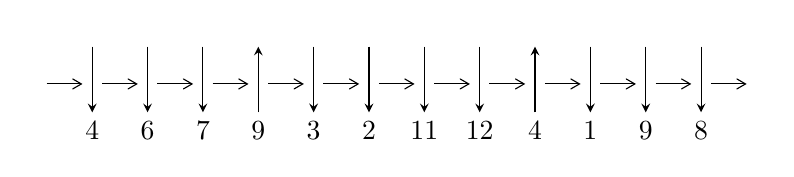
\begin{tikzpicture}[x=20pt, y=17pt]
	% nodes
	\node (C0) at (0, 0) {};
	\node (C1) at (1, 0) {};
	\node (C1U) at (1, +1) {};
	\node (C1D) at (1, -1) {4};

	\node (C2) at (2, 0) {};
	\node (C2U) at (2, +1) {};
	\node (C2D) at (2, -1) {6};

	\node (C3) at (3, 0) {};
	\node (C3U) at (3, +1) {};
	\node (C3D) at (3, -1) {7};

	\node (C4) at (4, 0) {};
	\node (C4U) at (4, +1) {};
	\node (C4D) at (4, -1) {9};

	\node (C5) at (5, 0) {};
	\node (C5U) at (5, +1) {};
	\node (C5D) at (5, -1) {3};

	\node (C6) at (6, 0) {};
	\node (C6U) at (6, +1) {};
	\node (C6D) at (6, -1) {2};

	\node (C7) at (7, 0) {};
	\node (C7U) at (7, +1) {};
	\node (C7D) at (7, -1) {11};

	\node (C8) at (8, 0) {};
	\node (C8U) at (8, +1) {};
	\node (C8D) at (8, -1) {12};

	\node (C9) at (9, 0) {};
	\node (C9U) at (9, +1) {};
	\node (C9D) at (9, -1) {4};

	\node (C10) at (10, 0) {};
	\node (C10U) at (10, +1) {};
	\node (C10D) at (10, -1) {1};

	\node (C11) at (11, 0) {};
	\node (C11U) at (11, +1) {};
	\node (C11D) at (11, -1) {9};

	\node (C12) at (12, 0) {};
	\node (C12U) at (12, +1) {};
	\node (C12D) at (12, -1) {8};
	\node (C13) at (13, 0) {};

	% arrows
	\draw[->,>={angle 60}]
	(C0) edge (C1) (C1) edge (C2) (C2) edge (C3) (C3) edge (C4) (C4) edge (C5) (C5) edge (C6) (C6) edge (C7) (C7) edge (C8) (C8) edge (C9) (C9) edge (C10) (C10) edge (C11) (C11) edge (C12) (C12) edge (C13) ;	\draw[->,>=stealth]
	(C1U) edge (C1D) (C2U) edge (C2D) (C3U) edge (C3D) (C4D) edge (C4U) (C5U) edge (C5D) (C6U) edge (C6D) (C7U) edge (C7D) (C8U) edge (C8D) (C9D) edge (C9U) (C10U) edge (C10D) (C11U) edge (C11D) (C12U) edge (C12D) ;
	\end{tikzpicture} \\
\hhline{~~} \\& 
\textbf{Solving Sequence} \\ \cline{2-2} 
 &
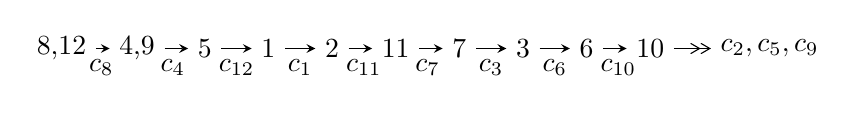
\begin{tikzpicture}[x=23pt, y=7pt]
	% node
	\node (A0) at (-1/8, 0) {8,12};
	\node (A1) at (17/16, 0) {4,9};
	\node (A2) at (17/8, 0) {5};
	\node (A3) at (25/8, 0) {1};
	\node (A4) at (33/8, 0) {2};
	\node (A5) at (41/8, 0) {11};
	\node (A6) at (49/8, 0) {7};
	\node (A7) at (57/8, 0) {3};
	\node (A8) at (65/8, 0) {6};
	\node (A9) at (73/8, 0) {10};
	\node (C1) at (1/2, -1) {$c_{8}$};
	\node (C2) at (13/8, -1) {$c_{4}$};
	\node (C3) at (21/8, -1) {$c_{12}$};
	\node (C4) at (29/8, -1) {$c_{1}$};
	\node (C5) at (37/8, -1) {$c_{11}$};
	\node (C6) at (45/8, -1) {$c_{7}$};
	\node (C7) at (53/8, -1) {$c_{3}$};
	\node (C8) at (61/8, -1) {$c_{6}$};
	\node (C9) at (69/8, -1) {$c_{10}$};
	\node (A10) at (11, 0) {$c_{2},c_{5},c_{9}$};

	% edge
	\draw[->,>=stealth]	
	(A0) edge (A1) (A1) edge (A2) (A2) edge (A3) (A3) edge (A4) (A4) edge (A5) (A5) edge (A6) (A6) edge (A7) (A7) edge (A8) (A8) edge (A9) ;
	\draw[->>,>={angle 60}]	
	(A9) edge (A10);
\end{tikzpicture} \\ 

\end{tabular} \\

\footnotetext{
The image of knot diagram is generated by the software ``\textbf{Draw programme}" developed by Andrew Bartholomew(\url{http://www.layer8.co.uk/maths/draw/index.htm\#Running-draw}), where we modified some parts for our purpose(\url{https://github.com/CATsTAILs/LinksPainter}).
}\phantom \\ \newline 
\centering \textbf{Ideals for irreducible components\footnotemark of $X_{\text{par}}$} 
 
\begin{align*}
I^u_{1}&=\langle 
u^5+u^4+2 u^3+2 u^2+b,\;- u^5- u^4-3 u^3-2 u^2+a-2 u,\\
\phantom{I^u_{1}}&\phantom{= \langle  }u^{10}+u^9+6 u^8+5 u^7+12 u^6+8 u^5+8 u^4+3 u^3+u^2-2 u+1\rangle \\
I^u_{2}&=\langle 
-2 u^{29}-3 u^{28}+\cdots+2 b+10,\;-13 u^{29}-37 u^{28}+\cdots+2 a+42,\;u^{30}+3 u^{29}+\cdots-8 u-1\rangle \\
I^u_{3}&=\langle 
u^2+b,\;a+1,\;u^3- u^2+2 u-1\rangle \\
I^u_{4}&=\langle 
- u^2 a+b,\;- u^2 a+a^2+u^2-2 a+2,\;u^3- u^2+2 u-1\rangle \\
\\
\end{align*}
\raggedright * 4 irreducible components of $\dim_{\mathbb{C}}=0$, with total 49 representations.\\
\footnotetext{All coefficients of polynomials are rational numbers. But the coefficients are sometimes approximated in decimal forms when there is not enough margin.}
\newpage
\renewcommand{\arraystretch}{1}
\centering \section*{I. $I^u_{1}= \langle u^5+u^4+2 u^3+2 u^2+b,\;- u^5- u^4-3 u^3-2 u^2+a-2 u,\;u^{10}+u^9+\cdots-2 u+1 \rangle$}
\flushleft \textbf{(i) Arc colorings}\\
\begin{tabular}{m{7pt} m{180pt} m{7pt} m{180pt} }
\flushright $a_{8}=$&$\begin{pmatrix}1\\0\end{pmatrix}$ \\
\flushright $a_{12}=$&$\begin{pmatrix}0\\u\end{pmatrix}$ \\
\flushright $a_{4}=$&$\begin{pmatrix}u^5+u^4+3 u^3+2 u^2+2 u\\- u^5- u^4-2 u^3-2 u^2\end{pmatrix}$ \\
\flushright $a_{9}=$&$\begin{pmatrix}1\\u^2\end{pmatrix}$ \\
\flushright $a_{5}=$&$\begin{pmatrix}- u^7- u^6-3 u^5-2 u^4- u^3+2 u\\- u^9- u^8-4 u^7-3 u^6-5 u^5-3 u^4-2 u^3-2 u^2\end{pmatrix}$ \\
\flushright $a_{1}=$&$\begin{pmatrix}- u\\u\end{pmatrix}$ \\
\flushright $a_{2}=$&$\begin{pmatrix}- u^9- u^8-5 u^7-4 u^6-8 u^5-4 u^4-4 u^3- u\\u^9+u^8+4 u^7+4 u^6+4 u^5+4 u^4+u\end{pmatrix}$ \\
\flushright $a_{11}=$&$\begin{pmatrix}u\\u^3+u\end{pmatrix}$ \\
\flushright $a_{7}=$&$\begin{pmatrix}- u^4- u^2+1\\- u^6-2 u^4- u^2\end{pmatrix}$ \\
\flushright $a_{3}=$&$\begin{pmatrix}u^7+3 u^5+u^4+3 u^3+2 u^2+u\\u^9+3 u^7+2 u^5- u^4- u^3-2 u^2\end{pmatrix}$ \\
\flushright $a_{6}=$&$\begin{pmatrix}- u^8- u^7-4 u^6-4 u^5-5 u^4-3 u^3- u^2+2 u\\2 u^8+u^7+7 u^6+4 u^5+6 u^4+3 u^3- u^2-2 u+1\end{pmatrix}$ \\
\flushright $a_{10}=$&$\begin{pmatrix}u^5+2 u^3+u\\- u^5- u^3+u\end{pmatrix}$\\&\end{tabular}
\flushleft \textbf{(ii) Obstruction class $= -1$}\\~\\
\flushleft \textbf{(iii) Cusp Shapes $= 4 u^9+4 u^8+22 u^7+22 u^6+42 u^5+40 u^4+30 u^3+20 u^2+8 u-10$}\\~\\
\newpage\renewcommand{\arraystretch}{1}
\flushleft \textbf{(iv) u-Polynomials at the component}\newline \\
\begin{tabular}{m{50pt}|m{274pt}}
Crossings & \hspace{64pt}u-Polynomials at each crossing \\
\hline $$\begin{aligned}c_{1},c_{10}\end{aligned}$$&$\begin{aligned}
&u^{10}- u^9+8 u^8-7 u^7+18 u^6-18 u^5+8 u^4-13 u^3+7 u^2+1
\end{aligned}$\\
\hline $$\begin{aligned}c_{2},c_{5},c_{6}\\c_{8},c_{11},c_{12}\end{aligned}$$&$\begin{aligned}
&u^{10}- u^9+6 u^8-5 u^7+12 u^6-8 u^5+8 u^4-3 u^3+u^2+2 u+1
\end{aligned}$\\
\hline $$\begin{aligned}c_{3},c_{7}\end{aligned}$$&$\begin{aligned}
&u^{10}+u^9+4 u^8+4 u^7+21 u^6-9 u^5+33 u^4+5 u^3+7 u^2+3 u+2
\end{aligned}$\\
\hline $$\begin{aligned}c_{4},c_{9}\end{aligned}$$&$\begin{aligned}
&u^{10}+7 u^9+\cdots+24 u+8
\end{aligned}$\\
\hline
\end{tabular}\\~\\
\newpage\renewcommand{\arraystretch}{1}
\flushleft \textbf{(v) Riley Polynomials at the component}\newline \\
\begin{tabular}{m{50pt}|m{274pt}}
Crossings & \hspace{64pt}Riley Polynomials at each crossing \\
\hline $$\begin{aligned}c_{1},c_{10}\end{aligned}$$&$\begin{aligned}
&y^{10}+15 y^9+\cdots+14 y+1
\end{aligned}$\\
\hline $$\begin{aligned}c_{2},c_{5},c_{6}\\c_{8},c_{11},c_{12}\end{aligned}$$&$\begin{aligned}
&y^{10}+11 y^9+\cdots-2 y+1
\end{aligned}$\\
\hline $$\begin{aligned}c_{3},c_{7}\end{aligned}$$&$\begin{aligned}
&y^{10}+7 y^9+\cdots+19 y+4
\end{aligned}$\\
\hline $$\begin{aligned}c_{4},c_{9}\end{aligned}$$&$\begin{aligned}
&y^{10}-7 y^9+\cdots+256 y+64
\end{aligned}$\\
\hline
\end{tabular}\\~\\
\newpage\flushleft \textbf{(vi) Complex Volumes and Cusp Shapes}
$$\begin{array}{c|c|c}  
\text{Solutions to }I^u_{1}& \I (\text{vol} + \sqrt{-1}CS) & \text{Cusp shape}\\
 \hline 
\begin{aligned}
u &= -0.728898 + 0.479191 I \\
a &= -0.415541 + 1.217980 I \\
b &= -0.927397 + 0.394143 I\end{aligned}
 & \phantom{-}5.65760 + 4.71262 I & -6.31236 - 5.61759 I \\ \hline\begin{aligned}
u &= -0.728898 - 0.479191 I \\
a &= -0.415541 - 1.217980 I \\
b &= -0.927397 - 0.394143 I\end{aligned}
 & \phantom{-}5.65760 - 4.71262 I & -6.31236 + 5.61759 I \\ \hline\begin{aligned}
u &= \phantom{-}0.066306 + 1.207890 I \\
a &= -0.854695 - 0.475151 I \\
b &= \phantom{-}0.697376 + 1.144550 I\end{aligned}
 & \phantom{-}5.29548 - 2.05211 I & -3.55200 + 3.27198 I \\ \hline\begin{aligned}
u &= \phantom{-}0.066306 - 1.207890 I \\
a &= -0.854695 + 0.475151 I \\
b &= \phantom{-}0.697376 - 1.144550 I\end{aligned}
 & \phantom{-}5.29548 + 2.05211 I & -3.55200 - 3.27198 I \\ \hline\begin{aligned}
u &= \phantom{-}0.11337 + 1.49042 I \\
a &= \phantom{-}1.075600 - 0.665737 I \\
b &= -1.60291 + 0.39329 I\end{aligned}
 & \phantom{-}11.32540 - 4.10290 I & \phantom{-}0.47358 + 2.87242 I \\ \hline\begin{aligned}
u &= \phantom{-}0.11337 - 1.49042 I \\
a &= \phantom{-}1.075600 + 0.665737 I \\
b &= -1.60291 - 0.39329 I\end{aligned}
 & \phantom{-}11.32540 + 4.10290 I & \phantom{-}0.47358 - 2.87242 I \\ \hline\begin{aligned}
u &= -0.28831 + 1.50977 I \\
a &= -2.00632 + 0.94362 I \\
b &= \phantom{-}3.37727 - 0.98896 I\end{aligned}
 & \phantom{-}18.5056 + 12.2668 I & -0.40879 - 5.71170 I \\ \hline\begin{aligned}
u &= -0.28831 - 1.50977 I \\
a &= -2.00632 - 0.94362 I \\
b &= \phantom{-}3.37727 + 0.98896 I\end{aligned}
 & \phantom{-}18.5056 - 12.2668 I & -0.40879 + 5.71170 I \\ \hline\begin{aligned}
u &= \phantom{-}0.337535 + 0.237080 I \\
a &= \phantom{-}0.700954 + 1.016800 I \\
b &= -0.044343 - 0.474934 I\end{aligned}
 & -0.483217 - 0.888721 I & -8.20043 + 7.80792 I \\ \hline\begin{aligned}
u &= \phantom{-}0.337535 - 0.237080 I \\
a &= \phantom{-}0.700954 - 1.016800 I \\
b &= -0.044343 + 0.474934 I\end{aligned}
 & -0.483217 + 0.888721 I & -8.20043 - 7.80792 I\\
 \hline 
 \end{array}$$\newpage\newpage\renewcommand{\arraystretch}{1}
\centering \section*{II. $I^u_{2}= \langle -2 u^{29}-3 u^{28}+\cdots+2 b+10,\;-13 u^{29}-37 u^{28}+\cdots+2 a+42,\;u^{30}+3 u^{29}+\cdots-8 u-1 \rangle$}
\flushleft \textbf{(i) Arc colorings}\\
\begin{tabular}{m{7pt} m{180pt} m{7pt} m{180pt} }
\flushright $a_{8}=$&$\begin{pmatrix}1\\0\end{pmatrix}$ \\
\flushright $a_{12}=$&$\begin{pmatrix}0\\u\end{pmatrix}$ \\
\flushright $a_{4}=$&$\begin{pmatrix}\frac{13}{2} u^{29}+\frac{37}{2} u^{28}+\cdots-\frac{209}{2} u-21\\u^{29}+\frac{3}{2} u^{28}+\cdots-\frac{43}{2} u-5\end{pmatrix}$ \\
\flushright $a_{9}=$&$\begin{pmatrix}1\\u^2\end{pmatrix}$ \\
\flushright $a_{5}=$&$\begin{pmatrix}\frac{15}{2} u^{29}+\frac{43}{2} u^{28}+\cdots-\frac{249}{2} u-25\\u^{29}+\frac{3}{2} u^{28}+\cdots-\frac{41}{2} u-5\end{pmatrix}$ \\
\flushright $a_{1}=$&$\begin{pmatrix}- u\\u\end{pmatrix}$ \\
\flushright $a_{2}=$&$\begin{pmatrix}- u^{29}-\frac{5}{2} u^{28}+\cdots+\frac{11}{2} u+\frac{5}{2}\\-\frac{1}{2} u^{27}- u^{26}+\cdots+3 u+\frac{1}{2}\end{pmatrix}$ \\
\flushright $a_{11}=$&$\begin{pmatrix}u\\u^3+u\end{pmatrix}$ \\
\flushright $a_{7}=$&$\begin{pmatrix}- u^4- u^2+1\\- u^6-2 u^4- u^2\end{pmatrix}$ \\
\flushright $a_{3}=$&$\begin{pmatrix}8 u^{29}+23 u^{28}+\cdots-142 u-\frac{57}{2}\\\frac{5}{2} u^{29}+5 u^{28}+\cdots-20 u-\frac{9}{2}\end{pmatrix}$ \\
\flushright $a_{6}=$&$\begin{pmatrix}7 u^{29}+19 u^{28}+\cdots-85 u-13\\\frac{1}{2} u^{29}-\frac{1}{2} u^{28}+\cdots-\frac{31}{2} u-3\end{pmatrix}$ \\
\flushright $a_{10}=$&$\begin{pmatrix}u^5+2 u^3+u\\- u^5- u^3+u\end{pmatrix}$\\&\end{tabular}
\flushleft \textbf{(ii) Obstruction class $= -1$}\\~\\
\flushleft \textbf{(iii) Cusp Shapes $= \frac{11}{2} u^{29}+15 u^{28}+\cdots-99 u-\frac{51}{2}$}\\~\\
\newpage\renewcommand{\arraystretch}{1}
\flushleft \textbf{(iv) u-Polynomials at the component}\newline \\
\begin{tabular}{m{50pt}|m{274pt}}
Crossings & \hspace{64pt}u-Polynomials at each crossing \\
\hline $$\begin{aligned}c_{1},c_{10}\end{aligned}$$&$\begin{aligned}
&u^{30}-3 u^{29}+\cdots-18 u^2+1
\end{aligned}$\\
\hline $$\begin{aligned}c_{2},c_{5},c_{6}\\c_{8},c_{11},c_{12}\end{aligned}$$&$\begin{aligned}
&u^{30}-3 u^{29}+\cdots+8 u-1
\end{aligned}$\\
\hline $$\begin{aligned}c_{3},c_{7}\end{aligned}$$&$\begin{aligned}
&u^{30}+3 u^{29}+\cdots+1074 u-153
\end{aligned}$\\
\hline $$\begin{aligned}c_{4},c_{9}\end{aligned}$$&$\begin{aligned}
&(u^{15}-3 u^{14}+\cdots-12 u+8)^{2}
\end{aligned}$\\
\hline
\end{tabular}\\~\\
\newpage\renewcommand{\arraystretch}{1}
\flushleft \textbf{(v) Riley Polynomials at the component}\newline \\
\begin{tabular}{m{50pt}|m{274pt}}
Crossings & \hspace{64pt}Riley Polynomials at each crossing \\
\hline $$\begin{aligned}c_{1},c_{10}\end{aligned}$$&$\begin{aligned}
&y^{30}+37 y^{29}+\cdots-36 y+1
\end{aligned}$\\
\hline $$\begin{aligned}c_{2},c_{5},c_{6}\\c_{8},c_{11},c_{12}\end{aligned}$$&$\begin{aligned}
&y^{30}+29 y^{29}+\cdots-20 y+1
\end{aligned}$\\
\hline $$\begin{aligned}c_{3},c_{7}\end{aligned}$$&$\begin{aligned}
&y^{30}+17 y^{29}+\cdots-192024 y+23409
\end{aligned}$\\
\hline $$\begin{aligned}c_{4},c_{9}\end{aligned}$$&$\begin{aligned}
&(y^{15}-21 y^{14}+\cdots+784 y-64)^{2}
\end{aligned}$\\
\hline
\end{tabular}\\~\\
\newpage\flushleft \textbf{(vi) Complex Volumes and Cusp Shapes}
$$\begin{array}{c|c|c}  
\text{Solutions to }I^u_{2}& \I (\text{vol} + \sqrt{-1}CS) & \text{Cusp shape}\\
 \hline 
\begin{aligned}
u &= -0.705981 + 0.612665 I \\
a &= -0.189821 + 0.894198 I \\
b &= -1.092990 + 0.473497 I\end{aligned}
 & \phantom{-}12.57910 - 3.33907 I & -2.38574 + 0.22991 I \\ \hline\begin{aligned}
u &= -0.705981 - 0.612665 I \\
a &= -0.189821 - 0.894198 I \\
b &= -1.092990 - 0.473497 I\end{aligned}
 & \phantom{-}12.57910 + 3.33907 I & -2.38574 - 0.22991 I \\ \hline\begin{aligned}
u &= -0.786126 + 0.466474 I \\
a &= \phantom{-}0.307960 - 1.352620 I \\
b &= \phantom{-}0.918649 - 0.316331 I\end{aligned}
 & \phantom{-}12.1008 + 8.3364 I & -3.32084 - 5.47194 I \\ \hline\begin{aligned}
u &= -0.786126 - 0.466474 I \\
a &= \phantom{-}0.307960 + 1.352620 I \\
b &= \phantom{-}0.918649 + 0.316331 I\end{aligned}
 & \phantom{-}12.1008 - 8.3364 I & -3.32084 + 5.47194 I \\ \hline\begin{aligned}
u &= -0.685541 + 0.538898 I \\
a &= \phantom{-}0.386781 - 0.997148 I \\
b &= \phantom{-}0.987952 - 0.464825 I\end{aligned}
 & \phantom{-}5.87309\phantom{ +0.000000I} & -5.59057 + 0. I\phantom{ +0.000000I} \\ \hline\begin{aligned}
u &= -0.685541 - 0.538898 I \\
a &= \phantom{-}0.386781 + 0.997148 I \\
b &= \phantom{-}0.987952 + 0.464825 I\end{aligned}
 & \phantom{-}5.87309\phantom{ +0.000000I} & -5.59057 + 0. I\phantom{ +0.000000I} \\ \hline\begin{aligned}
u &= \phantom{-}0.713656 + 0.166582 I \\
a &= -0.855543 - 0.376613 I \\
b &= \phantom{-}0.448037 + 0.280112 I\end{aligned}
 & \phantom{-}2.81581 - 0.87895 I & -5.63582 + 0.83931 I \\ \hline\begin{aligned}
u &= \phantom{-}0.713656 - 0.166582 I \\
a &= -0.855543 + 0.376613 I \\
b &= \phantom{-}0.448037 - 0.280112 I\end{aligned}
 & \phantom{-}2.81581 + 0.87895 I & -5.63582 - 0.83931 I \\ \hline\begin{aligned}
u &= \phantom{-}0.243602 + 1.279880 I \\
a &= \phantom{-}0.169871 + 0.426938 I \\
b &= \phantom{-}0.032440 - 0.551805 I\end{aligned}
 & \phantom{-}2.51678 - 3.17894 I & \phantom{-}0.37815 + 5.88971 I \\ \hline\begin{aligned}
u &= \phantom{-}0.243602 - 1.279880 I \\
a &= \phantom{-}0.169871 - 0.426938 I \\
b &= \phantom{-}0.032440 + 0.551805 I\end{aligned}
 & \phantom{-}2.51678 + 3.17894 I & \phantom{-}0.37815 - 5.88971 I\\
 \hline 
 \end{array}$$\newpage$$\begin{array}{c|c|c}  
\text{Solutions to }I^u_{2}& \I (\text{vol} + \sqrt{-1}CS) & \text{Cusp shape}\\
 \hline 
\begin{aligned}
u &= \phantom{-}0.302233 + 0.572979 I \\
a &= -0.891160 - 0.823170 I \\
b &= \phantom{-}0.029484 + 0.794061 I\end{aligned}
 & \phantom{-}4.68149 - 2.48936 I & -2.42897 + 4.40087 I \\ \hline\begin{aligned}
u &= \phantom{-}0.302233 - 0.572979 I \\
a &= -0.891160 + 0.823170 I \\
b &= \phantom{-}0.029484 - 0.794061 I\end{aligned}
 & \phantom{-}4.68149 + 2.48936 I & -2.42897 - 4.40087 I \\ \hline\begin{aligned}
u &= -0.029336 + 1.362430 I \\
a &= \phantom{-}1.53009 + 0.04314 I \\
b &= -2.06494 - 0.86724 I\end{aligned}
 & \phantom{-}2.81581 + 0.87895 I & -5.63582 - 0.83931 I \\ \hline\begin{aligned}
u &= -0.029336 - 1.362430 I \\
a &= \phantom{-}1.53009 - 0.04314 I \\
b &= -2.06494 + 0.86724 I\end{aligned}
 & \phantom{-}2.81581 - 0.87895 I & -5.63582 + 0.83931 I \\ \hline\begin{aligned}
u &= \phantom{-}0.635625\phantom{ +0.000000I} \\
a &= \phantom{-}0.526188\phantom{ +0.000000I} \\
b &= -0.268208\phantom{ +0.000000I}\end{aligned}
 & -1.48208\phantom{ +0.000000I} & -4.72100\phantom{ +0.000000I} \\ \hline\begin{aligned}
u &= \phantom{-}0.315927 + 1.335280 I \\
a &= \phantom{-}0.056628 - 0.761520 I \\
b &= -0.400717 + 0.793524 I\end{aligned}
 & \phantom{-}7.52431 - 4.63680 I & \phantom{-0.000000 -}0. + 2.51110 I \\ \hline\begin{aligned}
u &= \phantom{-}0.315927 - 1.335280 I \\
a &= \phantom{-}0.056628 + 0.761520 I \\
b &= -0.400717 - 0.793524 I\end{aligned}
 & \phantom{-}7.52431 + 4.63680 I & \phantom{-0.000000 } 0. - 2.51110 I \\ \hline\begin{aligned}
u &= \phantom{-}0.099338 + 1.386390 I \\
a &= -0.972274 + 0.248617 I \\
b &= \phantom{-}1.323920 + 0.164440 I\end{aligned}
 & \phantom{-}4.68149 - 2.48936 I & -2.42897 + 4.40087 I \\ \hline\begin{aligned}
u &= \phantom{-}0.099338 - 1.386390 I \\
a &= -0.972274 - 0.248617 I \\
b &= \phantom{-}1.323920 - 0.164440 I\end{aligned}
 & \phantom{-}4.68149 + 2.48936 I & -2.42897 - 4.40087 I \\ \hline\begin{aligned}
u &= -0.084417 + 1.399330 I \\
a &= -1.87882 + 0.15021 I \\
b &= \phantom{-}2.75314 + 0.68684 I\end{aligned}
 & \phantom{-}7.52431 + 4.63680 I & \phantom{-0.000000 } 0. - 2.51110 I\\
 \hline 
 \end{array}$$\newpage$$\begin{array}{c|c|c}  
\text{Solutions to }I^u_{2}& \I (\text{vol} + \sqrt{-1}CS) & \text{Cusp shape}\\
 \hline 
\begin{aligned}
u &= -0.084417 - 1.399330 I \\
a &= -1.87882 - 0.15021 I \\
b &= \phantom{-}2.75314 - 0.68684 I\end{aligned}
 & \phantom{-}7.52431 - 4.63680 I & \phantom{-0.000000 -}0. + 2.51110 I \\ \hline\begin{aligned}
u &= -0.26139 + 1.50518 I \\
a &= \phantom{-}2.03229 - 0.92308 I \\
b &= -3.40445 + 0.88020 I\end{aligned}
 & \phantom{-}12.1008 + 8.3364 I & \phantom{-0.000000 } 0. - 5.47194 I \\ \hline\begin{aligned}
u &= -0.26139 - 1.50518 I \\
a &= \phantom{-}2.03229 + 0.92308 I \\
b &= -3.40445 - 0.88020 I\end{aligned}
 & \phantom{-}12.1008 - 8.3364 I & \phantom{-0.000000 -}0. + 5.47194 I \\ \hline\begin{aligned}
u &= -0.23109 + 1.51730 I \\
a &= -2.02333 + 0.87807 I \\
b &= \phantom{-}3.32265 - 0.75494 I\end{aligned}
 & \phantom{-}12.57910 + 3.33907 I & \phantom{-0.000000 } 0 \\ \hline\begin{aligned}
u &= -0.23109 - 1.51730 I \\
a &= -2.02333 - 0.87807 I \\
b &= \phantom{-}3.32265 + 0.75494 I\end{aligned}
 & \phantom{-}12.57910 - 3.33907 I & \phantom{-0.000000 } 0 \\ \hline\begin{aligned}
u &= -0.21368 + 1.55326 I \\
a &= \phantom{-}1.97146 - 0.87493 I \\
b &= -3.15532 + 0.76228 I\end{aligned}
 & \phantom{-}19.7380\phantom{ +0.000000I} & \phantom{-0.000000 } 0 \\ \hline\begin{aligned}
u &= -0.21368 - 1.55326 I \\
a &= \phantom{-}1.97146 + 0.87493 I \\
b &= -3.15532 - 0.76228 I\end{aligned}
 & \phantom{-}19.7380\phantom{ +0.000000I} & \phantom{-0.000000 } 0 \\ \hline\begin{aligned}
u &= -0.354580 + 0.145881 I \\
a &= \phantom{-}2.47267 - 0.38301 I \\
b &= \phantom{-}0.785485 - 0.312110 I\end{aligned}
 & \phantom{-}2.51678 + 3.17894 I & \phantom{-}0.37815 - 5.88971 I \\ \hline\begin{aligned}
u &= -0.354580 - 0.145881 I \\
a &= \phantom{-}2.47267 + 0.38301 I \\
b &= \phantom{-}0.785485 + 0.312110 I\end{aligned}
 & \phantom{-}2.51678 - 3.17894 I & \phantom{-}0.37815 + 5.88971 I \\ \hline\begin{aligned}
u &= -0.280853\phantom{ +0.000000I} \\
a &= -2.75980\phantom{ +0.000000I} \\
b &= -0.698487\phantom{ +0.000000I}\end{aligned}
 & -1.48208\phantom{ +0.000000I} & -4.72100\phantom{ +0.000000I}\\
 \hline 
 \end{array}$$\newpage\newpage\renewcommand{\arraystretch}{1}
\centering \section*{III. $I^u_{3}= \langle u^2+b,\;a+1,\;u^3- u^2+2 u-1 \rangle$}
\flushleft \textbf{(i) Arc colorings}\\
\begin{tabular}{m{7pt} m{180pt} m{7pt} m{180pt} }
\flushright $a_{8}=$&$\begin{pmatrix}1\\0\end{pmatrix}$ \\
\flushright $a_{12}=$&$\begin{pmatrix}0\\u\end{pmatrix}$ \\
\flushright $a_{4}=$&$\begin{pmatrix}-1\\- u^2\end{pmatrix}$ \\
\flushright $a_{9}=$&$\begin{pmatrix}1\\u^2\end{pmatrix}$ \\
\flushright $a_{5}=$&$\begin{pmatrix}-1\\- u^2\end{pmatrix}$ \\
\flushright $a_{1}=$&$\begin{pmatrix}- u\\u\end{pmatrix}$ \\
\flushright $a_{2}=$&$\begin{pmatrix}- u^2-1\\u^2\end{pmatrix}$ \\
\flushright $a_{11}=$&$\begin{pmatrix}u\\u^2- u+1\end{pmatrix}$ \\
\flushright $a_{7}=$&$\begin{pmatrix}u\\- u\end{pmatrix}$ \\
\flushright $a_{3}=$&$\begin{pmatrix}u-2\\- u^2- u+1\end{pmatrix}$ \\
\flushright $a_{6}=$&$\begin{pmatrix}- u^2+2 u-1\\u^2-3 u+1\end{pmatrix}$ \\
\flushright $a_{10}=$&$\begin{pmatrix}1\\u^2\end{pmatrix}$\\&\end{tabular}
\flushleft \textbf{(ii) Obstruction class $= 1$}\\~\\
\flushleft \textbf{(iii) Cusp Shapes $= -8 u^2+8 u-20$}\\~\\
\newpage\renewcommand{\arraystretch}{1}
\flushleft \textbf{(iv) u-Polynomials at the component}\newline \\
\begin{tabular}{m{50pt}|m{274pt}}
Crossings & \hspace{64pt}u-Polynomials at each crossing \\
\hline $$\begin{aligned}c_{1},c_{3},c_{7}\\c_{10}\end{aligned}$$&$\begin{aligned}
&u^3+u^2-1
\end{aligned}$\\
\hline $$\begin{aligned}c_{2},c_{8}\end{aligned}$$&$\begin{aligned}
&u^3- u^2+2 u-1
\end{aligned}$\\
\hline $$\begin{aligned}c_{4},c_{9}\end{aligned}$$&$\begin{aligned}
&u^3
\end{aligned}$\\
\hline $$\begin{aligned}c_{5},c_{6},c_{11}\\c_{12}\end{aligned}$$&$\begin{aligned}
&u^3+u^2+2 u+1
\end{aligned}$\\
\hline
\end{tabular}\\~\\
\newpage\renewcommand{\arraystretch}{1}
\flushleft \textbf{(v) Riley Polynomials at the component}\newline \\
\begin{tabular}{m{50pt}|m{274pt}}
Crossings & \hspace{64pt}Riley Polynomials at each crossing \\
\hline $$\begin{aligned}c_{1},c_{3},c_{7}\\c_{10}\end{aligned}$$&$\begin{aligned}
&y^3- y^2+2 y-1
\end{aligned}$\\
\hline $$\begin{aligned}c_{2},c_{5},c_{6}\\c_{8},c_{11},c_{12}\end{aligned}$$&$\begin{aligned}
&y^3+3 y^2+2 y-1
\end{aligned}$\\
\hline $$\begin{aligned}c_{4},c_{9}\end{aligned}$$&$\begin{aligned}
&y^3
\end{aligned}$\\
\hline
\end{tabular}\\~\\
\newpage\flushleft \textbf{(vi) Complex Volumes and Cusp Shapes}
$$\begin{array}{c|c|c}  
\text{Solutions to }I^u_{3}& \I (\text{vol} + \sqrt{-1}CS) & \text{Cusp shape}\\
 \hline 
\begin{aligned}
u &= \phantom{-}0.215080 + 1.307140 I \\
a &= -1.00000\phantom{ +0.000000I} \\
b &= \phantom{-}1.66236 - 0.56228 I\end{aligned}
 & \phantom{-}6.04826 - 5.65624 I & -4.98049 + 5.95889 I \\ \hline\begin{aligned}
u &= \phantom{-}0.215080 - 1.307140 I \\
a &= -1.00000\phantom{ +0.000000I} \\
b &= \phantom{-}1.66236 + 0.56228 I\end{aligned}
 & \phantom{-}6.04826 + 5.65624 I & -4.98049 - 5.95889 I \\ \hline\begin{aligned}
u &= \phantom{-}0.569840\phantom{ +0.000000I} \\
a &= -1.00000\phantom{ +0.000000I} \\
b &= -0.324718\phantom{ +0.000000I}\end{aligned}
 & -2.22691\phantom{ +0.000000I} & -18.0390\phantom{ +0.000000I}\\
 \hline 
 \end{array}$$\newpage\newpage\renewcommand{\arraystretch}{1}
\centering \section*{IV. $I^u_{4}= \langle - u^2 a+b,\;- u^2 a+a^2+u^2-2 a+2,\;u^3- u^2+2 u-1 \rangle$}
\flushleft \textbf{(i) Arc colorings}\\
\begin{tabular}{m{7pt} m{180pt} m{7pt} m{180pt} }
\flushright $a_{8}=$&$\begin{pmatrix}1\\0\end{pmatrix}$ \\
\flushright $a_{12}=$&$\begin{pmatrix}0\\u\end{pmatrix}$ \\
\flushright $a_{4}=$&$\begin{pmatrix}a\\u^2 a\end{pmatrix}$ \\
\flushright $a_{9}=$&$\begin{pmatrix}1\\u^2\end{pmatrix}$ \\
\flushright $a_{5}=$&$\begin{pmatrix}a\\u^2 a\end{pmatrix}$ \\
\flushright $a_{1}=$&$\begin{pmatrix}- u\\u\end{pmatrix}$ \\
\flushright $a_{2}=$&$\begin{pmatrix}- u^2 a+a u+u^2-2 a-2 u+2\\- a u+2 u\end{pmatrix}$ \\
\flushright $a_{11}=$&$\begin{pmatrix}u\\u^2- u+1\end{pmatrix}$ \\
\flushright $a_{7}=$&$\begin{pmatrix}u\\- u\end{pmatrix}$ \\
\flushright $a_{3}=$&$\begin{pmatrix}- a u+2 a\\u^2 a+a u- a\end{pmatrix}$ \\
\flushright $a_{6}=$&$\begin{pmatrix}-2 u^2 a+2 a u+3 u^2-2 a- u+4\\2 u^2 a-2 a u- u^2+a\end{pmatrix}$ \\
\flushright $a_{10}=$&$\begin{pmatrix}1\\u^2\end{pmatrix}$\\&\end{tabular}
\flushleft \textbf{(ii) Obstruction class $= 1$}\\~\\
\flushleft \textbf{(iii) Cusp Shapes $= 3 u^2 a-5 a u-3 u^2+3 a+3 u-12$}\\~\\
\newpage\renewcommand{\arraystretch}{1}
\flushleft \textbf{(iv) u-Polynomials at the component}\newline \\
\begin{tabular}{m{50pt}|m{274pt}}
Crossings & \hspace{64pt}u-Polynomials at each crossing \\
\hline $$\begin{aligned}c_{1},c_{3},c_{7}\\c_{10}\end{aligned}$$&$\begin{aligned}
&(u^3+u^2-1)^2
\end{aligned}$\\
\hline $$\begin{aligned}c_{2},c_{8}\end{aligned}$$&$\begin{aligned}
&(u^3- u^2+2 u-1)^2
\end{aligned}$\\
\hline $$\begin{aligned}c_{4},c_{9}\end{aligned}$$&$\begin{aligned}
&u^6
\end{aligned}$\\
\hline $$\begin{aligned}c_{5},c_{6},c_{11}\\c_{12}\end{aligned}$$&$\begin{aligned}
&(u^3+u^2+2 u+1)^2
\end{aligned}$\\
\hline
\end{tabular}\\~\\
\newpage\renewcommand{\arraystretch}{1}
\flushleft \textbf{(v) Riley Polynomials at the component}\newline \\
\begin{tabular}{m{50pt}|m{274pt}}
Crossings & \hspace{64pt}Riley Polynomials at each crossing \\
\hline $$\begin{aligned}c_{1},c_{3},c_{7}\\c_{10}\end{aligned}$$&$\begin{aligned}
&(y^3- y^2+2 y-1)^2
\end{aligned}$\\
\hline $$\begin{aligned}c_{2},c_{5},c_{6}\\c_{8},c_{11},c_{12}\end{aligned}$$&$\begin{aligned}
&(y^3+3 y^2+2 y-1)^2
\end{aligned}$\\
\hline $$\begin{aligned}c_{4},c_{9}\end{aligned}$$&$\begin{aligned}
&y^6
\end{aligned}$\\
\hline
\end{tabular}\\~\\
\newpage\flushleft \textbf{(vi) Complex Volumes and Cusp Shapes}
$$\begin{array}{c|c|c}  
\text{Solutions to }I^u_{4}& \I (\text{vol} + \sqrt{-1}CS) & \text{Cusp shape}\\
 \hline 
\begin{aligned}
u &= \phantom{-}0.215080 + 1.307140 I \\
a &= -0.162359 + 0.986732 I \\
b &= -0.28492 - 1.73159 I\end{aligned}
 & \phantom{-}6.04826\phantom{ +0.000000I} &                  -6
-1.085931 + 0. 10   I\phantom{ +0.000000I} \\ \hline\begin{aligned}
u &= \phantom{-}0.215080 + 1.307140 I \\
a &= \phantom{-}0.500000 - 0.424452 I \\
b &= -0.592519 + 0.986732 I\end{aligned}
 & \phantom{-}1.91067 - 2.82812 I & -9.95703 + 1.11003 I \\ \hline\begin{aligned}
u &= \phantom{-}0.215080 - 1.307140 I \\
a &= -0.162359 - 0.986732 I \\
b &= -0.28492 + 1.73159 I\end{aligned}
 & \phantom{-}6.04826\phantom{ +0.000000I} &                  -6
-1.085931 + 0. 10   I\phantom{ +0.000000I} \\ \hline\begin{aligned}
u &= \phantom{-}0.215080 - 1.307140 I \\
a &= \phantom{-}0.500000 + 0.424452 I \\
b &= -0.592519 - 0.986732 I\end{aligned}
 & \phantom{-}1.91067 + 2.82812 I & -9.95703 - 1.11003 I \\ \hline\begin{aligned}
u &= \phantom{-}0.569840\phantom{ +0.000000I} \\
a &= \phantom{-}1.16236 + 0.98673 I \\
b &= \phantom{-}0.377439 + 0.320410 I\end{aligned}
 & \phantom{-}1.91067 - 2.82812 I & -9.95703 + 1.11003 I \\ \hline\begin{aligned}
u &= \phantom{-}0.569840\phantom{ +0.000000I} \\
a &= \phantom{-}1.16236 - 0.98673 I \\
b &= \phantom{-}0.377439 - 0.320410 I\end{aligned}
 & \phantom{-}1.91067 + 2.82812 I & -9.95703 - 1.11003 I\\
 \hline 
 \end{array}$$\newpage
\newpage\renewcommand{\arraystretch}{1}
\centering \section*{ V. u-Polynomials}
\begin{tabular}{m{50pt}|m{274pt}}
Crossings & \hspace{64pt}u-Polynomials at each crossing \\
\hline $$\begin{aligned}c_{1},c_{10}\end{aligned}$$&$\begin{aligned}
&(u^3+u^2-1)^3\\
&\cdot(u^{10}- u^9+8 u^8-7 u^7+18 u^6-18 u^5+8 u^4-13 u^3+7 u^2+1)\\
&\cdot(u^{30}-3 u^{29}+\cdots-18 u^2+1)
\end{aligned}$\\
\hline $$\begin{aligned}c_{2},c_{8}\end{aligned}$$&$\begin{aligned}
&(u^3- u^2+2 u-1)^3\\
&\cdot(u^{10}- u^9+6 u^8-5 u^7+12 u^6-8 u^5+8 u^4-3 u^3+u^2+2 u+1)\\
&\cdot(u^{30}-3 u^{29}+\cdots+8 u-1)
\end{aligned}$\\
\hline $$\begin{aligned}c_{3},c_{7}\end{aligned}$$&$\begin{aligned}
&(u^3+u^2-1)^3\\
&\cdot(u^{10}+u^9+4 u^8+4 u^7+21 u^6-9 u^5+33 u^4+5 u^3+7 u^2+3 u+2)\\
&\cdot(u^{30}+3 u^{29}+\cdots+1074 u-153)
\end{aligned}$\\
\hline $$\begin{aligned}c_{4},c_{9}\end{aligned}$$&$\begin{aligned}
&u^9(u^{10}+7 u^9+\cdots+24 u+8)(u^{15}-3 u^{14}+\cdots-12 u+8)^{2}
\end{aligned}$\\
\hline $$\begin{aligned}c_{5},c_{6},c_{11}\\c_{12}\end{aligned}$$&$\begin{aligned}
&(u^3+u^2+2 u+1)^3\\
&\cdot(u^{10}- u^9+6 u^8-5 u^7+12 u^6-8 u^5+8 u^4-3 u^3+u^2+2 u+1)\\
&\cdot(u^{30}-3 u^{29}+\cdots+8 u-1)
\end{aligned}$\\
\hline
\end{tabular}\newpage\renewcommand{\arraystretch}{1}
\centering \section*{ VI. Riley Polynomials}
\begin{tabular}{m{50pt}|m{274pt}}
Crossings & \hspace{64pt}Riley Polynomials at each crossing \\
\hline $$\begin{aligned}c_{1},c_{10}\end{aligned}$$&$\begin{aligned}
&((y^3- y^2+2 y-1)^3)(y^{10}+15 y^9+\cdots+14 y+1)\\
&\cdot(y^{30}+37 y^{29}+\cdots-36 y+1)
\end{aligned}$\\
\hline $$\begin{aligned}c_{2},c_{5},c_{6}\\c_{8},c_{11},c_{12}\end{aligned}$$&$\begin{aligned}
&((y^3+3 y^2+2 y-1)^3)(y^{10}+11 y^9+\cdots-2 y+1)\\
&\cdot(y^{30}+29 y^{29}+\cdots-20 y+1)
\end{aligned}$\\
\hline $$\begin{aligned}c_{3},c_{7}\end{aligned}$$&$\begin{aligned}
&((y^3- y^2+2 y-1)^3)(y^{10}+7 y^9+\cdots+19 y+4)\\
&\cdot(y^{30}+17 y^{29}+\cdots-192024 y+23409)
\end{aligned}$\\
\hline $$\begin{aligned}c_{4},c_{9}\end{aligned}$$&$\begin{aligned}
&y^9(y^{10}-7 y^9+\cdots+256 y+64)(y^{15}-21 y^{14}+\cdots+784 y-64)^{2}
\end{aligned}$\\
\hline
\end{tabular}
\vskip 2pc
\end{document}